\newif\ifpaper

%\papertrue

\ifpaper
	\documentclass[ignorenonframetext,handout,english]{beamer}
	\usepackage{pgfpages}
	\pgfpagesuselayout{2 on 1}[a4paper,border shrink=5mm]
\else
	\documentclass[english]{beamer}
\fi

% A4 paper
\usepackage[T1]{fontenc}
\usepackage{babel}
\usepackage{beamerthemesplit}
\usepackage[latin2]{inputenc}
\usepackage{url}
\usetheme{Dresden}
\usecolortheme[rgb={0.3, 0.3, 0.9}]{structure}

\title{Software Renderer \\Accelerated by CUDA Technology}
\author{Wojciech Sterna}
\date{25th of January, 2011}



\begin{document}



\frame{\titlepage}



\section{Introduction}

\frame
{
	\frametitle{Fundamental Concepts}
	{
		\begin{itemize}
			\pause
			\item rendering --- process of generating a 2D image from a 3D data set
			\pause
			\item the graphics pipeline --- set of stages the input 3D data set is passed through to generate the 2D output image
			\pause
			\item CUDA --- technology from NVIDIA that allows for parallel general-purpose code execution using graphics cards
		\end{itemize}
	}
}

\frame
{
	\frametitle{Goals of the Work}
	{
		\begin{itemize}
			\pause
			\item implement in software a selected subset of OpenGL --- Vainmoinen
			\pause
			\item speed the implementation with CUDA
			\pause
			\item compare the performance of a reference application using:
				\begin{itemize}
					\item Vainmoinen without CUDA
					\item Vainmoinen with CUDA
					\item OpenGL
				\end{itemize}
		\end{itemize}
	}
}



\section{The Graphics Pipeline}

\frame
{
	\frametitle{World Definition}
	{
		\pause

		\begin{itemize}
			\item the world is built with triangles only
			\item every triangle consists of 3 vertices
			\item every vertex has a position, color and texture coordinate
		\end{itemize}
	}
}

\frame
{
	\frametitle{Vertex Processing}
	{
		\pause

		\begin{itemize}
			\item input vertex $P = (x, y, z)$ goes through a series of matrix transformations resulting in vertex $P' = (x', y', z')$, where:
				\begin{itemize}
					\item $(x', y')$ --- position of the vertex on the screen in window coordinates
					\item $z'$ --- distance of the vertex to the camera in normalized $[-1, 1]$ range
				\end{itemize}
		\end{itemize}

		\pause

		Other operations that take place during vertex processing:

		\begin{itemize}
			\item clipping to the near plane
			\item view frustum culling
			\item backface culling
		\end{itemize}
	}
}

\frame
{
	\frametitle{Pixel Processing}
	{
		\pause

		\begin{itemize}
			\item loop through the pixels of every triangle
			\item use barycentric coordinates to get the interpolated values (color and texture coordinate) at every pixel, given the values at the vertices of the triangle being processed
		\end{itemize}
	}
}

\frame
{
	\frametitle{Pixel Processing}
	{
		Naive interpolation leads to incorrectly rendered image:

		\begin{figure}
		\centering
		
\includegraphics[scale=0.6]{interpolation_a.png}
		\end{figure}

		\pause

		Solution --- perspective-correct interpolation:

		\begin{figure}
		\centering
		
\includegraphics[scale=0.6]{interpolation_b.png}
		\end{figure}
	}
}

\frame
{
	\frametitle{Pixel Processing}
	{
		Texture magnification:

		\begin{figure}
		\centering
		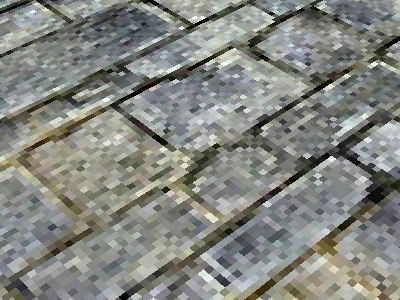
\includegraphics[scale=0.25]{sampling_point.png}
		\end{figure}

		\pause

		Solution --- bilinear filtering:

		\begin{figure}
		\centering
		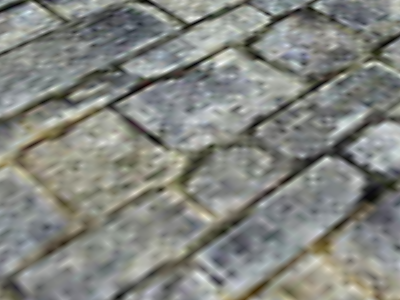
\includegraphics[scale=0.25]{sampling_bilinear.png}
		\end{figure}
	}
}

\frame
{
	\frametitle{Pixel Processing}
	{
		Texture minification:

		\begin{figure}
		\centering
		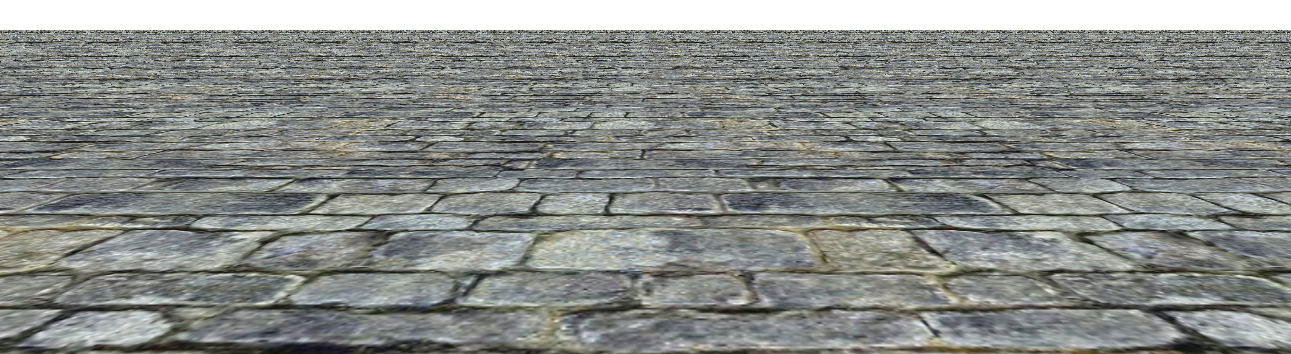
\includegraphics[scale=0.25]{mipmaps_off.png}
		\end{figure}

		\pause

		Solution --- mipmapping:

		\begin{figure}
		\centering
		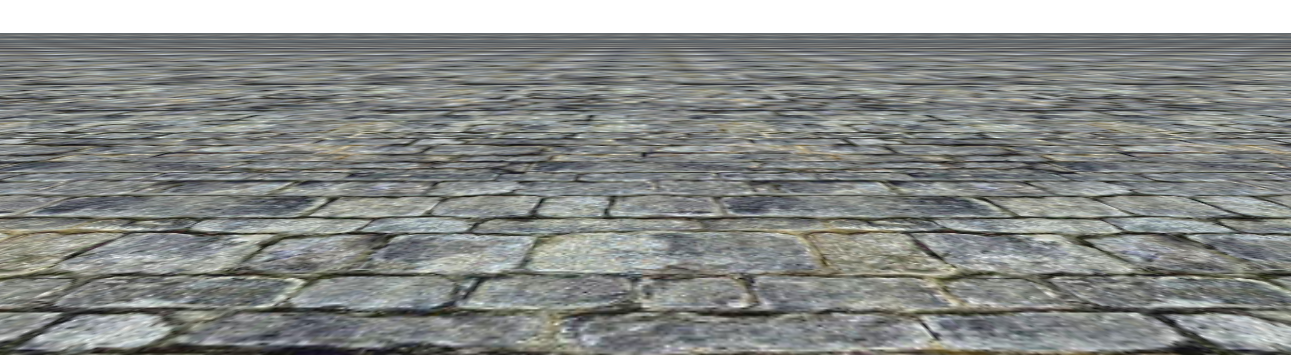
\includegraphics[scale=0.25]{mipmaps_on.png}
		\end{figure}
	}
}



\section{Project Architecture}

\frame
{
	\frametitle{UML Class Diagram}
	{
		\begin{figure}
		\centering
		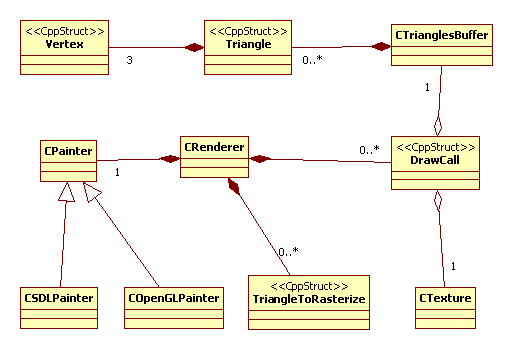
\includegraphics[scale=0.5]{class_diagram.png}
		\end{figure}
	}
}



\section{Demo}

\frame
{
	\frametitle{Demo}
	{
		\begin{figure}
		\centering
		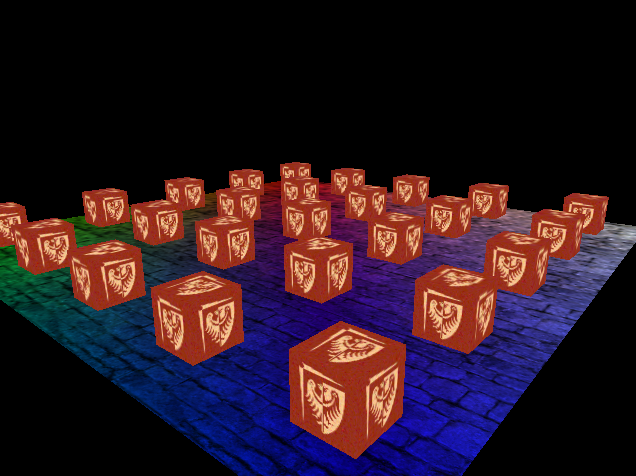
\includegraphics[scale=0.5]{demo.png}
		\end{figure}
	}
}



\section{Performance Tests}

\frame
{
	\frametitle{Performance Tests}
	{
		\pause

		Test 1 --- a few of huge triangles:

		\begin{center}
			\begin{tabular}{| l | c |}
			\hline
			\textbf{Renderer} & \textbf{Time} \\ \hline \hline
			Vainmoinen without CUDA & 10400 ms \\ \hline
			Vainmoinen with CUDA (One-Call-One-Triangle) & 225 ms \\ \hline
			Vainmoinen with CUDA (One-Call-Many-Triangles) & 2200 ms \\ \hline
			OpenGL & 32 ms \\ \hline
			\end{tabular}
		\end{center}

		\pause

		Test 2 --- a lot of tiny triangles:

		\begin{center}
			\begin{tabular}{| l | c |}
			\hline
			\textbf{Renderer} & \textbf{Time} \\ \hline \hline
			Vainmoinen without CUDA & 24 ms \\ \hline
			Vainmoinen with CUDA (One-Call-One-Triangle) & 415 ms \\ \hline
			Vainmoinen with CUDA (One-Call-Many-Triangles) & 33 ms \\ \hline
			OpenGL & 22 ms \\ \hline
			\end{tabular}
		\end{center}
	}
}



\section{Conclusions and Future Work}

\frame
{
	\frametitle{Conclusions and Future Work}
	{
		\begin{itemize}
			\pause
			\item implementation of the renderer itself has proven \textbf{not to be} that difficult
			\pause
			\item gaining the mathematical background needed to know how to implement the renderer has proven \textbf{to be} difficult \\
			\pause
			it was also a great fun by the way
			\pause
			\item CUDA can greatly speed up calculations
			\pause
			\item further development of Vainmoinen would simply involve implementation of additional features
		\end{itemize}
	}
}



\section*{}

\frame
{
	Thank you for the attention!
}



\end{document}
